\section{File System Provisioning and System Monitoring}

This section describes the file system provisioning and system monitoring
subsystems of \ngrm.  By coupling these systems to the resource manager,
we achieve our goals of mitigating system noise, improving job launch time,
and promoting reproduceability and data provenance.

\subsection{File System Provisioning}

We use the term "file system provisioning" to describe how executables
and other read-only data are provided to compute nodes.
A provisioning system based on immutable datasets is proposed.
Immutable datasets are collections of files that can be aggressively cached
without revalidation,
and reliably referenced in a job record for data provenance.
In the proposed system, a dataset is stored in a container,
actually itself a file formatted as a local file system such as ext4 or
squashfs.  The container, which is stored in a special dataset repository,
is exported as a read-only network block device,
then mounted like a regular local file system on compute nodes,
where the files that comprise the dataset are individually accessible.
The system can be used to provision the root file system,
or any other file system provided its content can be stored immutably
in a dataset container and managed in the dataset repository.

The provisioning system consists of the
distributed network block device,
dataset repository,
tools for creating and managing datasets,
and the resource manager interfaces for assigning datasets to jobs
such that they become part of a job's runtime environment and
are referenced in the job's historical record.


\subsubsection{Distributed Network Block Device}

A network block device driver based on 9P protocol called 9nbd\cite{9nbd}
was prototyped in August 2012.
9nbd, which at a high level has functionality similar to iSCSI or SRP,
leverages the existing kernel 9P transport to access a backing file
in a remote 9P file system.
A hierarcically distributed, shared network block device can be built
using 9nbd and any number of levels of chained 9P diod\cite{diod}
I/O forwarding servers, fanned out in a hierarchy as depicted in
Figure~\ref{Fig9nbd}.
\begin{figure}
\centering
\fbox{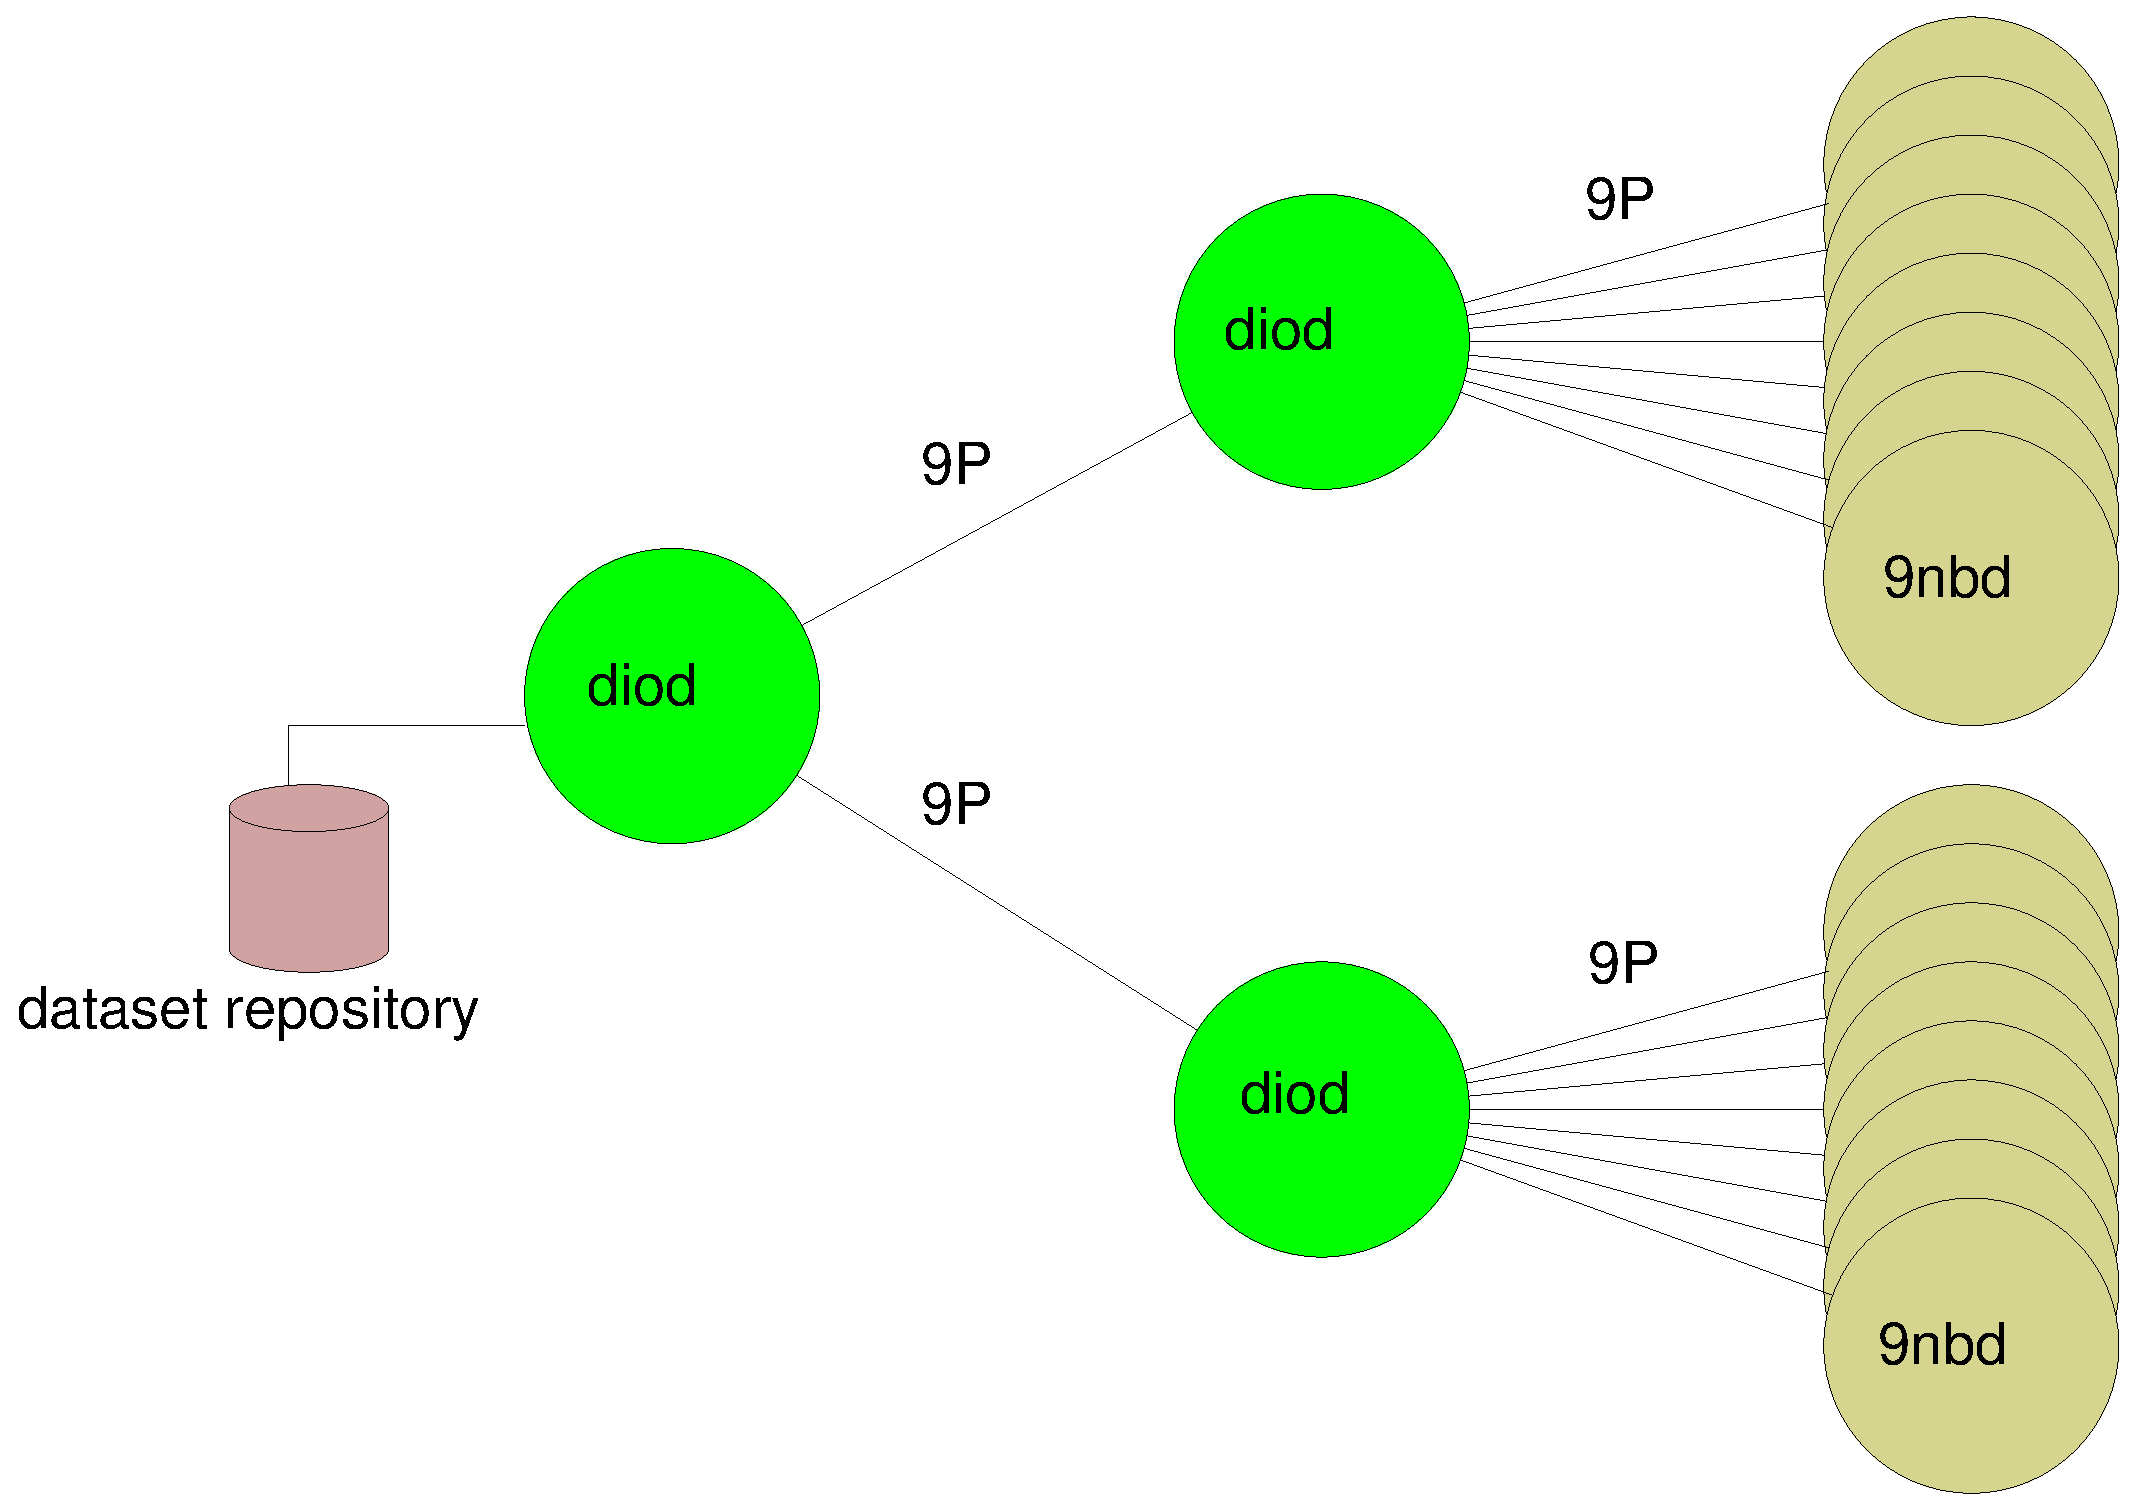
\includegraphics[scale=0.30]{../fig/dnbd.eps}}
\caption{
Immutable, read-only datasets residing in repository are forwarded by diod
I/O forwarding server to compute nodes running 9nbd where they appear
as block devices.  Block devices are mounted on compute nodes with
the semantics of a local file system.
}
\label{Fig9nbd}
\end{figure}

\paragraph{Performance Outlook}
A diod I/O forwarding server will read the working set of the container
file in once and thereafter serve it from its page cache to multiple clients.
At each compute node,
the block device driver naturally caches its working set in the buffer cache,
which is optimized for many common file system usage patterns,
such as path search and dynamic library loading.
A study of parallel path search\cite{BlkDevPathSearch}
using ext4, the {\em loopback} block device, one level of diod I/O forwarding
with a fanout of 82 to 1, and a single NFS server,
showed flat scaling to 82 nodes, the largest scale attempted,
while NFS began to slow at eight nodes.
This result, depicted in Figure~\ref{FigPathWalk},
indicates that the distributed block device based on 9P has
great promise to improve job launch times over NFS, and the flexible
hierarchical architecture should easily scale to 100K nodes, although
testing with more than one level of diod forwarding may identify some
additional work required to get there.
\begin{figure}
\centering
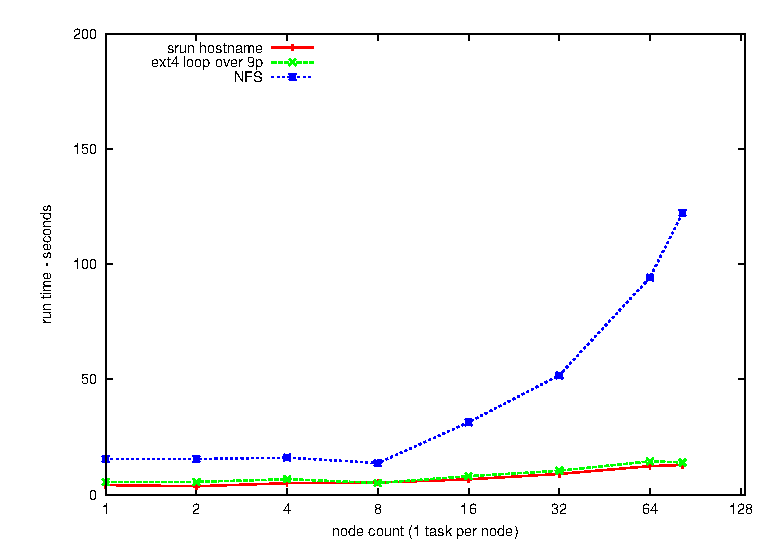
\includegraphics[scale=1]{../fig/pathwalk.eps}
\caption{
Path walk performance for distributed block device based on 9P and diod
scales the same as the null slurm job up to 82 nodes, while NFS begins
to slow at 8 nodes.
}
\label{FigPathWalk}
\end{figure}

\paragraph{System Noise Outlook}
The distributed block device requires no cache management as the
data is read-only throughout the system.  Unlike NFS (even mounted read-only),
compute nodes will not attempt to asynchronously revalidate cached
attributes or data, since the entire dataset is immutable.
Data in the buffer cache is never dirty, and can be thrown out and at
any point should the application require the memory, and reread on demand later.
Therefore, the approach is very friendly to applications running on compute
nodes, with a system noise footprint that can be near zero.

\paragraph{Security}
The 9nbd prototype and diod server implement MUNGE authentication
over the built-in TCP transport plugin, and no integrity or privacy.
The \ngrm\ comms framework security model should be leveraged,
by adding an \ngrm-specific kernel 9P transport plugin,
to obtain integrity and privacy for I/O forwarding within a comms session,

\paragraph{Resiliency}
The 9nbd prototype implements single server resiliency, where the
9nbd block device driver can re-establish the transport and replay
9P connection state to a new server instance should the server reboot.
The client blocks while this recovery takes place.
The \ngrm\ comms framework CMB should be leveraged,
by adding an \ngrm-specific kernel 9P transport plugin,
to obtain multi-server resiliency based on storing possible diod server
identities in the CMB state and tracking liveness changes.
The client can thus recover more quickly by leveraging the CMB.

\paragraph{Root File System Special Needs}
Provisioning the system root file system to diskless nodes requires
some additional care and is somewhat distribution specific.
Root has to be mounted from a limited initramfs environment, which
implies that MUNGE and 9nbd have to be functional in that environment.
For distributions based on Red Hat Enterprise Linux, a {\em dracut}
module is needed for both MUNGE and 9nbd.  Once root is mounted, it can
remain read-only, or more conveniently, it can be combined with a {\em zram}
memory-based block device using {\em dm-snapshot}, making it appear
writable, with any changes going to RAM.  The dracut modules and the
dm-snapshot/zram support can be added to the nfsroot\cite{nfsroot}
software package.

\subsubsection{Dataset Repository}

Dataset containers can initially be stored in NFS, Lustre, or a local file
system and managed by system administrators using simple scripts.
However, there are a few practical problems with this.
One is that a large number of nearly identical containers may proliferate
and use too much space.  Another is that there is no mechanism to enforce
the immutability of a dataset under a given file name, and no way
to incorporate job record references (e.g. a use count) into a repository
purge policy.
Finally, the intent is to allow users to manage the content of their datasets,
but user access must be controlled such that containers are always
valid file system images and container metadata is properly filled in.
These three factors motivate the need for a specialized dataset repository.

\paragraph{Copy-on-write}
A large number of nearly identical containers may proliferate, for example
if a dataset is undergoing iterative changes during development.
Ideally the file system storing dataset containers will support
{\em thin copies} or block level {\em de-duplication} so that only one
copy of unchanged content is stored.

\paragraph{Content Addressable}
To prevent datasets from changing while mounted, which would trigger
kernel panics, and from run to run, which would affect provenance and
reproduceability, the file system storing dataset containers should
be content addressable.  For example, instead of a file name, a cryptographic
hash of its content is used to refer to a container file.
The file system or the repository interface should enforce this atomically.

\paragraph{Container Format and Repository Model}
Containers must contain valid file system images in order to avoid
mount errors or kernel panics, and certain metadata should be associated
with containers to record information about how it was created.
The resource manager will take references on containers when they are used
and when they are referenced by a job's provenance record.
Thus the dataset repository is more than a file system that has
content addressability and copy-on-write.
It must enforce provisioning system policy over container additions and
removals and ensure that all its containers have a valid format.

\subsubsection{Tools for Creating and Managing Datasets}

Tools similar to those provided for package management are required to
create valid containers with proper metadata from collections of files,
for managing and updating containers, and for interacting with the repository.
Stakeholders such as system administrators and code teams who might
be interested in creating datasets should be consulted to understand
their workflow and tool needs.  

\subsubsection{Resource Manager Interface}

The provisioning system is intended to be used in conjunction with
the \ngrm\ runtime's capability of configuring the file system
namespace (e.g. set of mount points) on a custom basis for each job. 

FIXME: launching a custom I/O forwarding topology within the job
vs fixed topology.

FIXME: taking a reference on a container while it is mounted and
from job log for provenance.

\subsubsection{File System Provisioning WBS}

\begin{longtable}{|p{1cm}|p{10.2cm}|p{1cm}|p{1cm}|p{1.8cm}|}\hline
  \textbf{Item} & \textbf{Description}
                & \textbf{Deliv}\footnote{SD = software drop,
                        DR = design review, V = viewgraphs, D = document}
                & \textbf{Weeks} & \textbf{Depend} \\
  \hline
  \hline
  \multicolumn{5}{|l|}{3.1. \textbf{Distributed Network Block Device}} \\
  \hline
  3.1.1.& Complete initial 9nbd network block device development, including
          backport upstream 9P transport fixes, refine/test 9nbd resiliency
          code, submit for LKML integration.
        & SD
        & 
        & \\
  \hline
  3.1.2.& (root file system only) Add MUNGE key bootstrap and 9nbd root
	  support to nfsroot dracut module.
        & SD
        & 
        & \\
  \hline
  3.1.3.& (root file system only) Backport zram TRIM support so space
	  can be reclaimed in zram-based root file systems.
        & SD
        & 
        & \\
  \hline
  3.1.4.& Design/develop initial container format and rudimentary scripts
	  for creating containers for manually managed NFS dataset repository.
        & SD
        & 
        & \\
  \hline
  3.1.5.& Production release of distributed network block device
	  with root file system support.
	  Support booting up to 4000 nodes from a container stored
	  on a Netapp NFS filer, and forwarded via one level of diod
	  I/O forwarding.
	  Implement single node resiliency and MUNGE authentication
	  (no privacy or integrity).
        & SD
        & 
        & 3.1.1, 3.1.2, 3.1.3, 3.1.4\\
  \hline
  3.1.6.& Performance study at scale of direct NFS vs distributed block
	    device, including Pynamic, pathwalk, and FTQ.
        & V
        & 
        & 3.1.5 \\
  \hline
  3.1.7.& Explore best way to remount multiple levels of diod servers.
          Use v9fs with cache=loose?  Is more work needed to allow
	  arbitrary levels of I/O forwarding?
        & V
        & 
        & \\
  \hline
  3.1.8.& Design/prototype 9P transport plugin that leverages the \ngrm\ 
	  comms framework for resiliency and privacy/integrity.
        & DR
        & 
        & \\
  \hline
  3.1.9.& Implement 9P transport plugin.
        & SD
        & 
        & 3.1.8\\
  \hline
  \multicolumn{5}{|l|}{3.2. \textbf{Dataset Repository, Tools, and \ngrm\ Integration}} \\
  \hline
  3.2.1.& Design/prototype SLURM SPANK plugin that allows users
          to select among available root images.  Manage private file system
          namespace for user, perform post-mount configuration, perform uid
          mapping.  Develop strategy for handling mounts such as home
          directories that would be overmounted by a new root.
        & DR
        & 
        & 3.1.5 \\
  \hline
  3.2.2.& Design/prototype container format and tools for
	  creating/managing datasets.
	  Consult with stakeholders to understand workflow.
	  Demo prototype and iterate.
        & DR
        & 
        & \\
  \hline
  3.2.3.& Design/prototype dataset repository with copy-on-write/dedup,
	  content addressability, repo contract enforcement.
        & DR
        & 
        & \\
  \hline
  3.2.4.& Implement tools for creating/managing datasets.
        & SD
        & 
        & 3.2.2 \\
  \hline
  3.2.5.& Implement dataset repository.
        & SD
        & 
        & 3.2.3 \\
  \hline
  3.2.6.& Design/prototype \ngrm\ integration including
	  private file system namespace management,
          RM management of dataset references during execution and in job
	  record,
	  RM launch of private diod daemons.
	  (co-design with \ngrm\ runtime?)
        & DR
        & 
        & 3.1.5, 3.2.1, 3.2.3, 3.2.4 \\
  \hline
  3.2.7.& Implement \ngrm\ integration.
        & SD
        & 
        & 3.2.6 \\
  \hline
\end{longtable}
\newpage

\subsection{System Monitoring}

\ngrm\ system monitoring consists of three main components:
a plugin system which allows user and system defined code to execute
periodically to check for anomolous situations or take data samples,
a monitoring console which aggregates the state of resources within a
comms sesssion and presents it in the form of a web page for users and
support staff, and a NoSQL monitoring database used to store data for
offline analysis and data provenance.
These subsystems are layered upon the comms framework event messaging and
aggregation/reduction services.  The general approach is to allow monitoring
to be customized within a session, with the parent session delegating
the responsibility for monitoring to its children.

\subsubsection{Monitoring Plugin System}

The monitoring plugin system provides a facility for arbitrary code to be
periodically executed across a session.  To minimize disruption to
bulk-synchronous workloads, this execution is synchronized by the 
session scheduling trigger event.  The set of active plugins is
under the control of the session owner, with some reasonable
defaults provided that can be overridden.

The details of the plugin structure is a design activity, however,
an example of a possible solution is for plugins to take the form of
Lua scripts loaded into the CMB state database
(thus shared across the session) and executed in the context of
a monitoring daemon with an embedded Lua interpreter.

Plugins have three main functions: data source, data reduction,
and data sink.  The data source function is driven by the scheduling
trigger and may directly publish events, for example if a monitored
value exceeds a threshold, or produce structured data for the
aggregation/reduction network.
The data reduction function aggregates structured data from instances
of the plugin's source function.
For example, a plugin that monitors the total amount of memory used
by the session might register a reduction function that takes the sum of
arriving samples.
Finally, plugins can register a function to sink data at the monitoring
console, rendering it for display, or at points in the session that interface
with the NoSQL monitoring database for persistent storage.

\subsubsection{Monitoring Console}

The monitoring console runs on the session control node and provides
a centralized point for monitoring each session.
An HTTP interface is provided which includes links to the control nodes
of child sessions, thus the entire hierarchy of sessions can be navigated
from the root session with a web browser.
The console displays information about the session that comes directly
from the comms CMB, including its time of inception, node membership,
node liveness, users, and scheduling trigger period.

The set of active plugins and the views created by them are represented.
Events generated by plugins are displayed in a scrollable region.

All the information that is available via the monitoring console web page
is also available via command line tools to a shell user on the session
control node.

\subsubsection{NoSQL Monitoring Database}

The NoSQL monitoring database is a large, centralized, persistent database
that stores structured log data for analysis and data provenance.
Log data is generated by monitoring plugins, but may come from other sources
such as syslog, the \ngrm\ runtime, resource manager, or scheduler.

One reason this database is centralized is to allow queries
to be constructed that correlate failures or performance anomalies
across domains; for example, jobs running slow or producing incorrect
results because of file system problems.  The database will directly
benefit system administrators and suport staff who currently perform
these tasks manually.

By preserving contextual information surrounding the execution of a job,
we enable questions to be asked later on when the same job produces
different results.  This is a central goal of provenance.

The database will need some schema design in order to enable queries
that are operationally useful.  For example, RAS metrics may be obtained
on hardware component failures if we are careful to log enough information
to identify the component (e.g. a double bit memory error at address \#xxxx
versus a failure of dimm with model and serial number).

This effort will leverage the work of an in-progress LDRD
feasbility study\cite{LogLDRD}.

\subsubsection{Monitoring WBS}

\begin{longtable}{|p{1cm}|p{10.2cm}|p{1cm}|p{1cm}|p{1.8cm}|}\hline
  \textbf{Item} & \textbf{Description}
                & \textbf{Deliv}\footnote{SD = software drop,
                        DR = design review, V = viewgraphs, D = document}
                & \textbf{Weeks} & \textbf{Depend} \\
  \hline
  \hline
  \multicolumn{5}{|l|}{3.3. \textbf{Monitoring Plugin System}} \\
  \hline
  3.3.1.& Design/prototype plugin system including structured log format
	  and event naming.  (See also possible CIFTS/FTB tie-in in runtime).
          (See also Meyer monitoring project).
	& DR
	&
	& \\
  \hline
  3.3.2.& Implement plugin system.
        & SD
        &
        & 3.3.1 \\
  \hline
  3.3.3.& Document process for creating monitoring plugins.
        & D
        &
        & 3.3.1 \\
  \hline
  3.3.4.& Design/prototype a set of default plugins including plugins
          for instrumenting jobs to gather "implicit provenance" such as
          file accesses.
        & DR
        & 
        & 3.3.1 \\
  \hline
  3.3.5 & Implement set of default plugins.
        & SD
        &
        & 3.3.4 \\

  \hline
  \multicolumn{5}{|l|}{3.4. \textbf{Monitoring Console}} \\
  \hline

  3.4.1.& Design/prototype HTTP/REST monitoring console.
          (Long/Martinez Lorenz team)
          (See also Meyer monitoring project).
	& DR
	&
	& 3.3.1 \\
  \hline
  3.4.2.& Implement monitoring console.
	& SD
	&
	& 3.3.1, 3.4.1 \\
  \hline
  3.4.3.& Design/prototype Lorenz integration.
	  Think about how monitoring console integrates with the myllnl
	  dashboard experience.
          (Long/Martinez Lorenz team)
	& DR
	&
	& 3.4.1 \\
  \hline
  3.4.4.& Design/prototype skummee integration.
          How will \ngrm\ integrate with ops monitoring view?
          How will out of band monitoring (IPMI, DDN's, etc) integrate with
	  monitoring console?
          (Meyer monitoring project).
	& DR
	&
	& 3.4.1 \\
  \hline
  3.4.5.& Implement Lorenz/skummee integration.
	& SD
	&
	& 3.4.3, 3.4.4 \\
  \hline
  \multicolumn{5}{|l|}{3.5. \textbf{NoSQL Monitoring Database}} \\
  \hline
  3.5.1.& Study available NoSQL databases for 100K node scalability
          and appropriate query interface.
          Use offline log data to investigate system diagnostic capability
          and prototype queries.
          (Gamblin/Mohror HPC Data Analytics FY12 LDRD)
        & V
        & 
        & LDRD \\
  \hline
  3.5.2.& Implement prototype database tied to live log sources.
          Study scalability and develop queries.
          (Gamblin/Mohror HPC Data Analytics FY12 LDRD)
          (See also: Faaland SPLUNK deployment).
        & DR
        & 
        & 3.5.1 \\
  \hline
  3.5.3.& Design/prototype access-role based security.
        & DR
        & 
        & 3.5.2 \\
  \hline
  3.5.4.& Design/prototype schemas and queries for reporting
          RAS metrics of interest to center management.
        & DR
        & 
        & 3.5.2 \\
  \hline
  3.5.5.& Design/prototype procedure for sanitizing and releasing data
	  for research study and citation.
        & DR
        & 
        & 3.5.2 \\
  \hline
  3.5.6.& Design/prototype schema for job logs and queries for
          associating job data, system log data, etc..
        & DR
        & 
        & RM, 3.5.2 \\
  \hline
  3.5.7.& Implement database.
        & SD
        & 
        & 3.5.2, 3.5.3, 3.5.4, 3.5.5, 3.5.6 \\
  \hline
\end{longtable}


